\subsect{Sprint 2}{sprint2}

\underline{Fecha de inicio}: 11/07/2022

\underline{Fecha de fin}: 11/08/2022

\underline{Objetivos}:
\begin{itemize}
	\item Mantener un historial de mensajes por cada chat.
	\item Añadir mejoras de seguridad.
\end{itemize}

\underline{Descripción}:
En este sprint se pretende añadir un historial de mensajes por cada chat, de forma que se pueda acceder a los
mensajes anteriores.\ Además, se añadirán mejoras de seguridad a la aplicación, como por ejemplo, la
encriptación de las contraseñas de los usuarios utilizando otro algoritmo más seguro.\ También se añadirá un sistema
de permisos para los usuarios, de forma que se pueda restringir el acceso a ciertas funcionalidades de la aplicación.

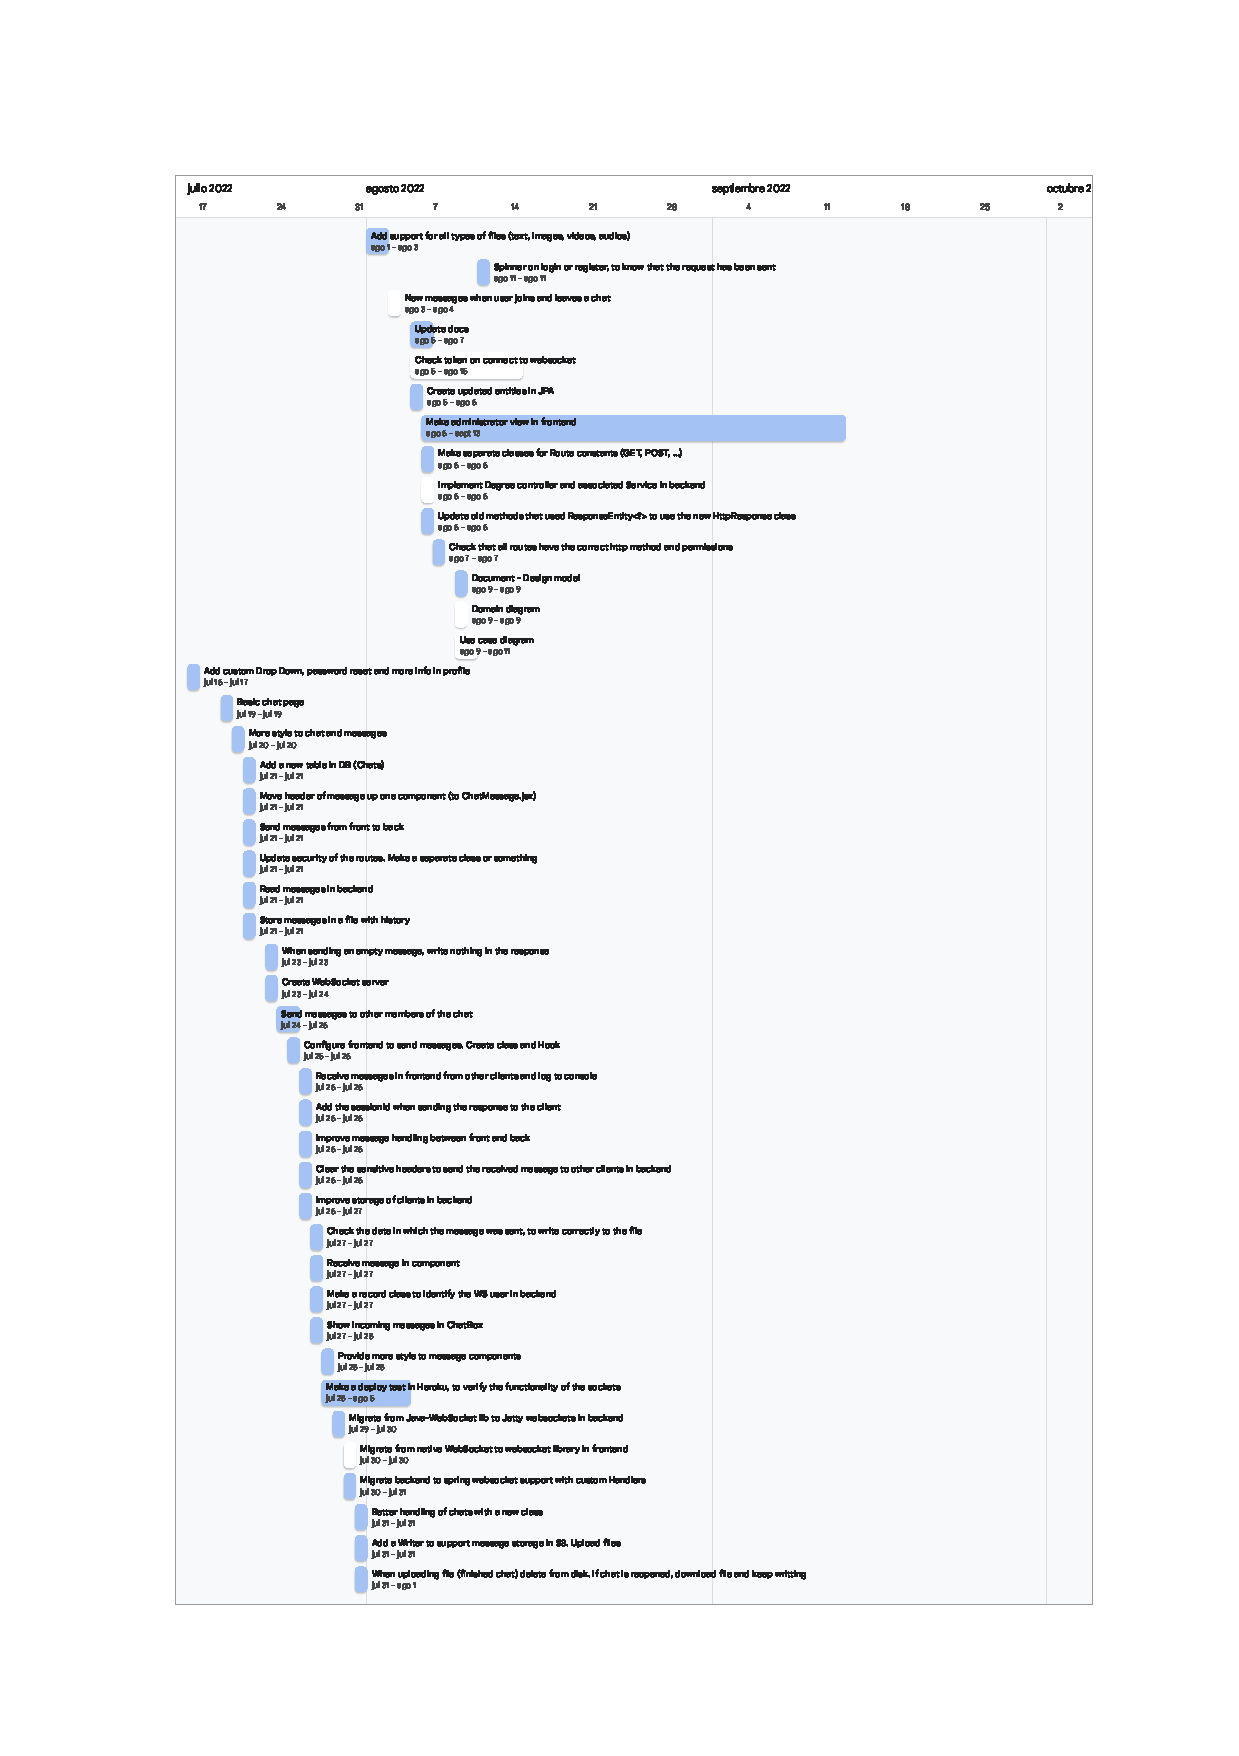
\includepdf[pages=-]{backlog/sprints/Sprint2.pdf}
